% F06: Correlation network graph (edges for |r| >= 0.30)
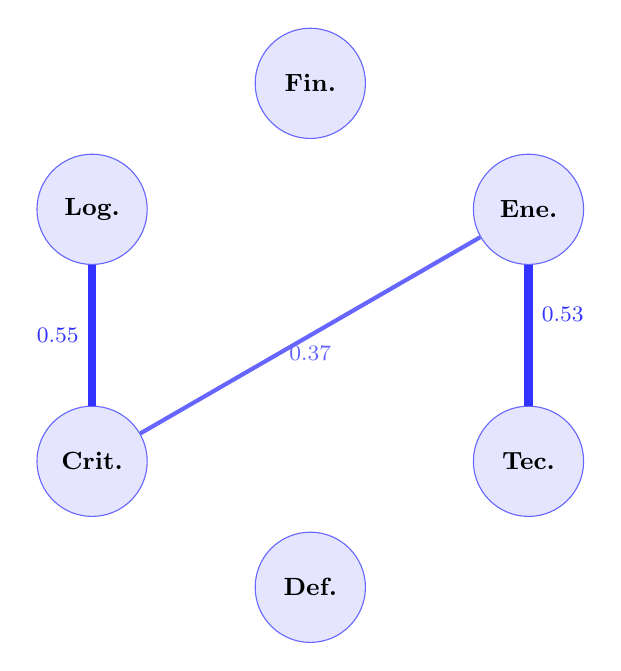
\begin{tikzpicture}[
  node distance=3cm,
  axisnode/.style={circle, draw=blue!60, fill=blue!10,
    minimum size=1.4cm, font=\small\bfseries, align=center},
  edge30/.style={line width=1.5pt, blue!60},
  edge50/.style={line width=3.0pt, blue!80},
]
% Place nodes in a hexagonal layout
\node[axisnode] (fin) at (90:3.2cm)  {Fin.};
\node[axisnode] (ene) at (30:3.2cm)  {Ene.};
\node[axisnode] (tec) at (330:3.2cm) {Tec.};
\node[axisnode] (def) at (270:3.2cm) {Def.};
\node[axisnode] (cri) at (210:3.2cm) {Crit.};
\node[axisnode] (log) at (150:3.2cm) {Log.};

% Edges with |r| >= 0.30
% Energy -- Technology:  r = 0.530
\draw[edge50] (ene) -- (tec) node[midway, above right, font=\footnotesize] {0.53};
% Energy -- Critical:    r = 0.372
\draw[edge30] (ene) -- (cri) node[midway, below, font=\footnotesize] {0.37};
% Critical -- Logistics: r = 0.549
\draw[edge50] (cri) -- (log) node[midway, left, font=\footnotesize] {0.55};
% Note: no other pair exceeds 0.30
\end{tikzpicture}
